% !TeX root = ../presentation.tex

\section{Intra-Urban Heat Island Effect}
\begin{frame}{What is the intra-urban heat island effect?}
	\begin{columns}[T] % align columns
		\begin{column}{.48\textwidth}
			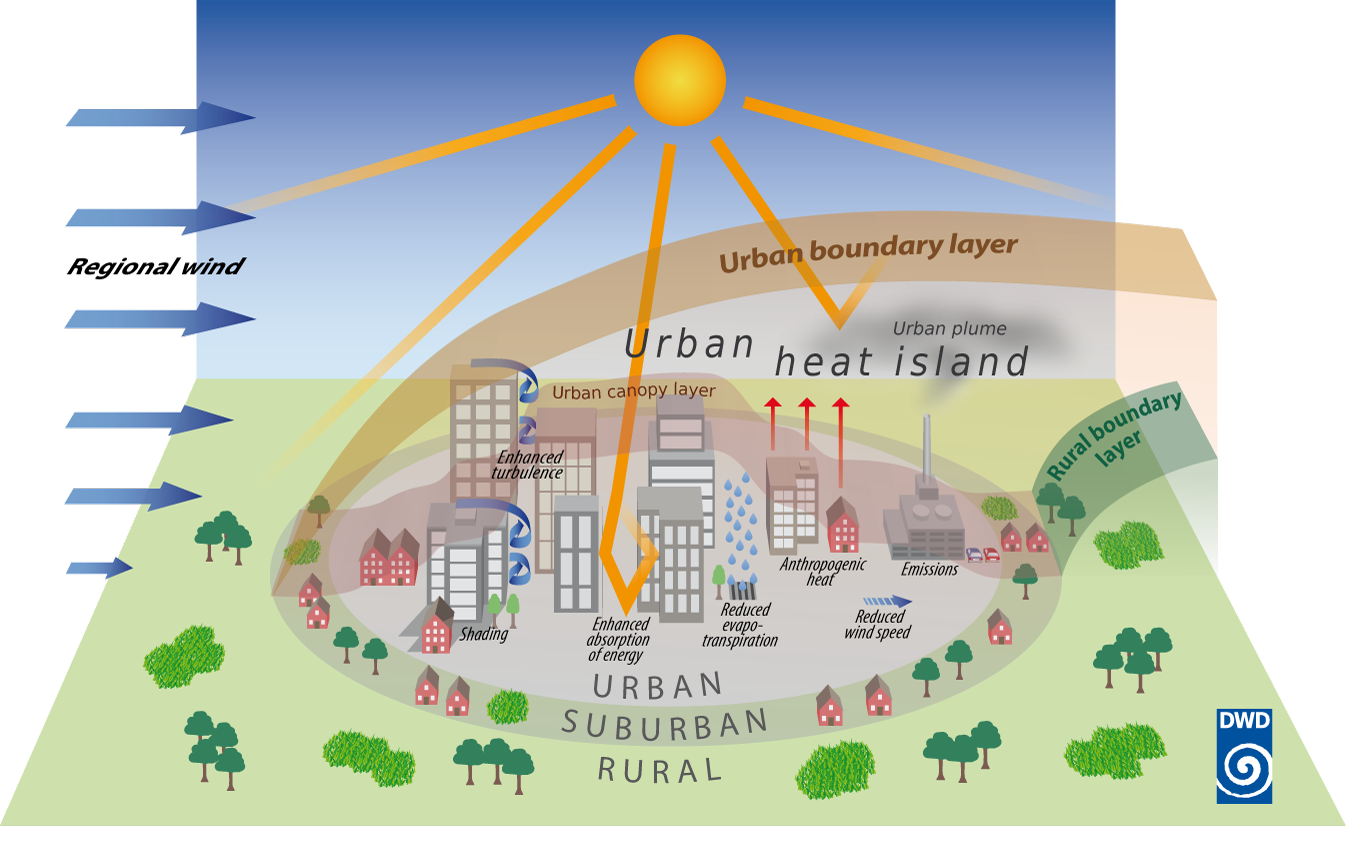
\includegraphics[width=\linewidth]{images/urbanheatisland_01.png}\\
			\textit{\footnotesize Source: Deutscher Wetterdienst\\Urban climate - urban heat islands}
		\end{column}%
		\hfill%
		\begin{column}{.56\textwidth}
			\begin{itemize}
				\item \glqq{}{[\textellipsis]} an urban area or metropolitan area is significantly warmer than its surrounding rural areas due to human activities\grqq{}\cite{takebayashi_chapter_2020}
				\item Infrastructure, such as buildings, roads and other sealed surfaces absorb and re-emit the sun's radiation in the form of heat
				\item natural landscapes, such as forests and water bodies have a cooling effect\cite{us_epa_learn_2014}
			\end{itemize}
		\end{column}%
	\end{columns}
\end{frame}
\begin{frame}{This is interpolation!}
	\begin{columns}[T] % align columns
		\begin{column}{.56\textwidth}
			\begin{itemize}
				\item TODO
			\end{itemize}
		\end{column}%
		\hfill%
		\begin{column}{.48\textwidth}
			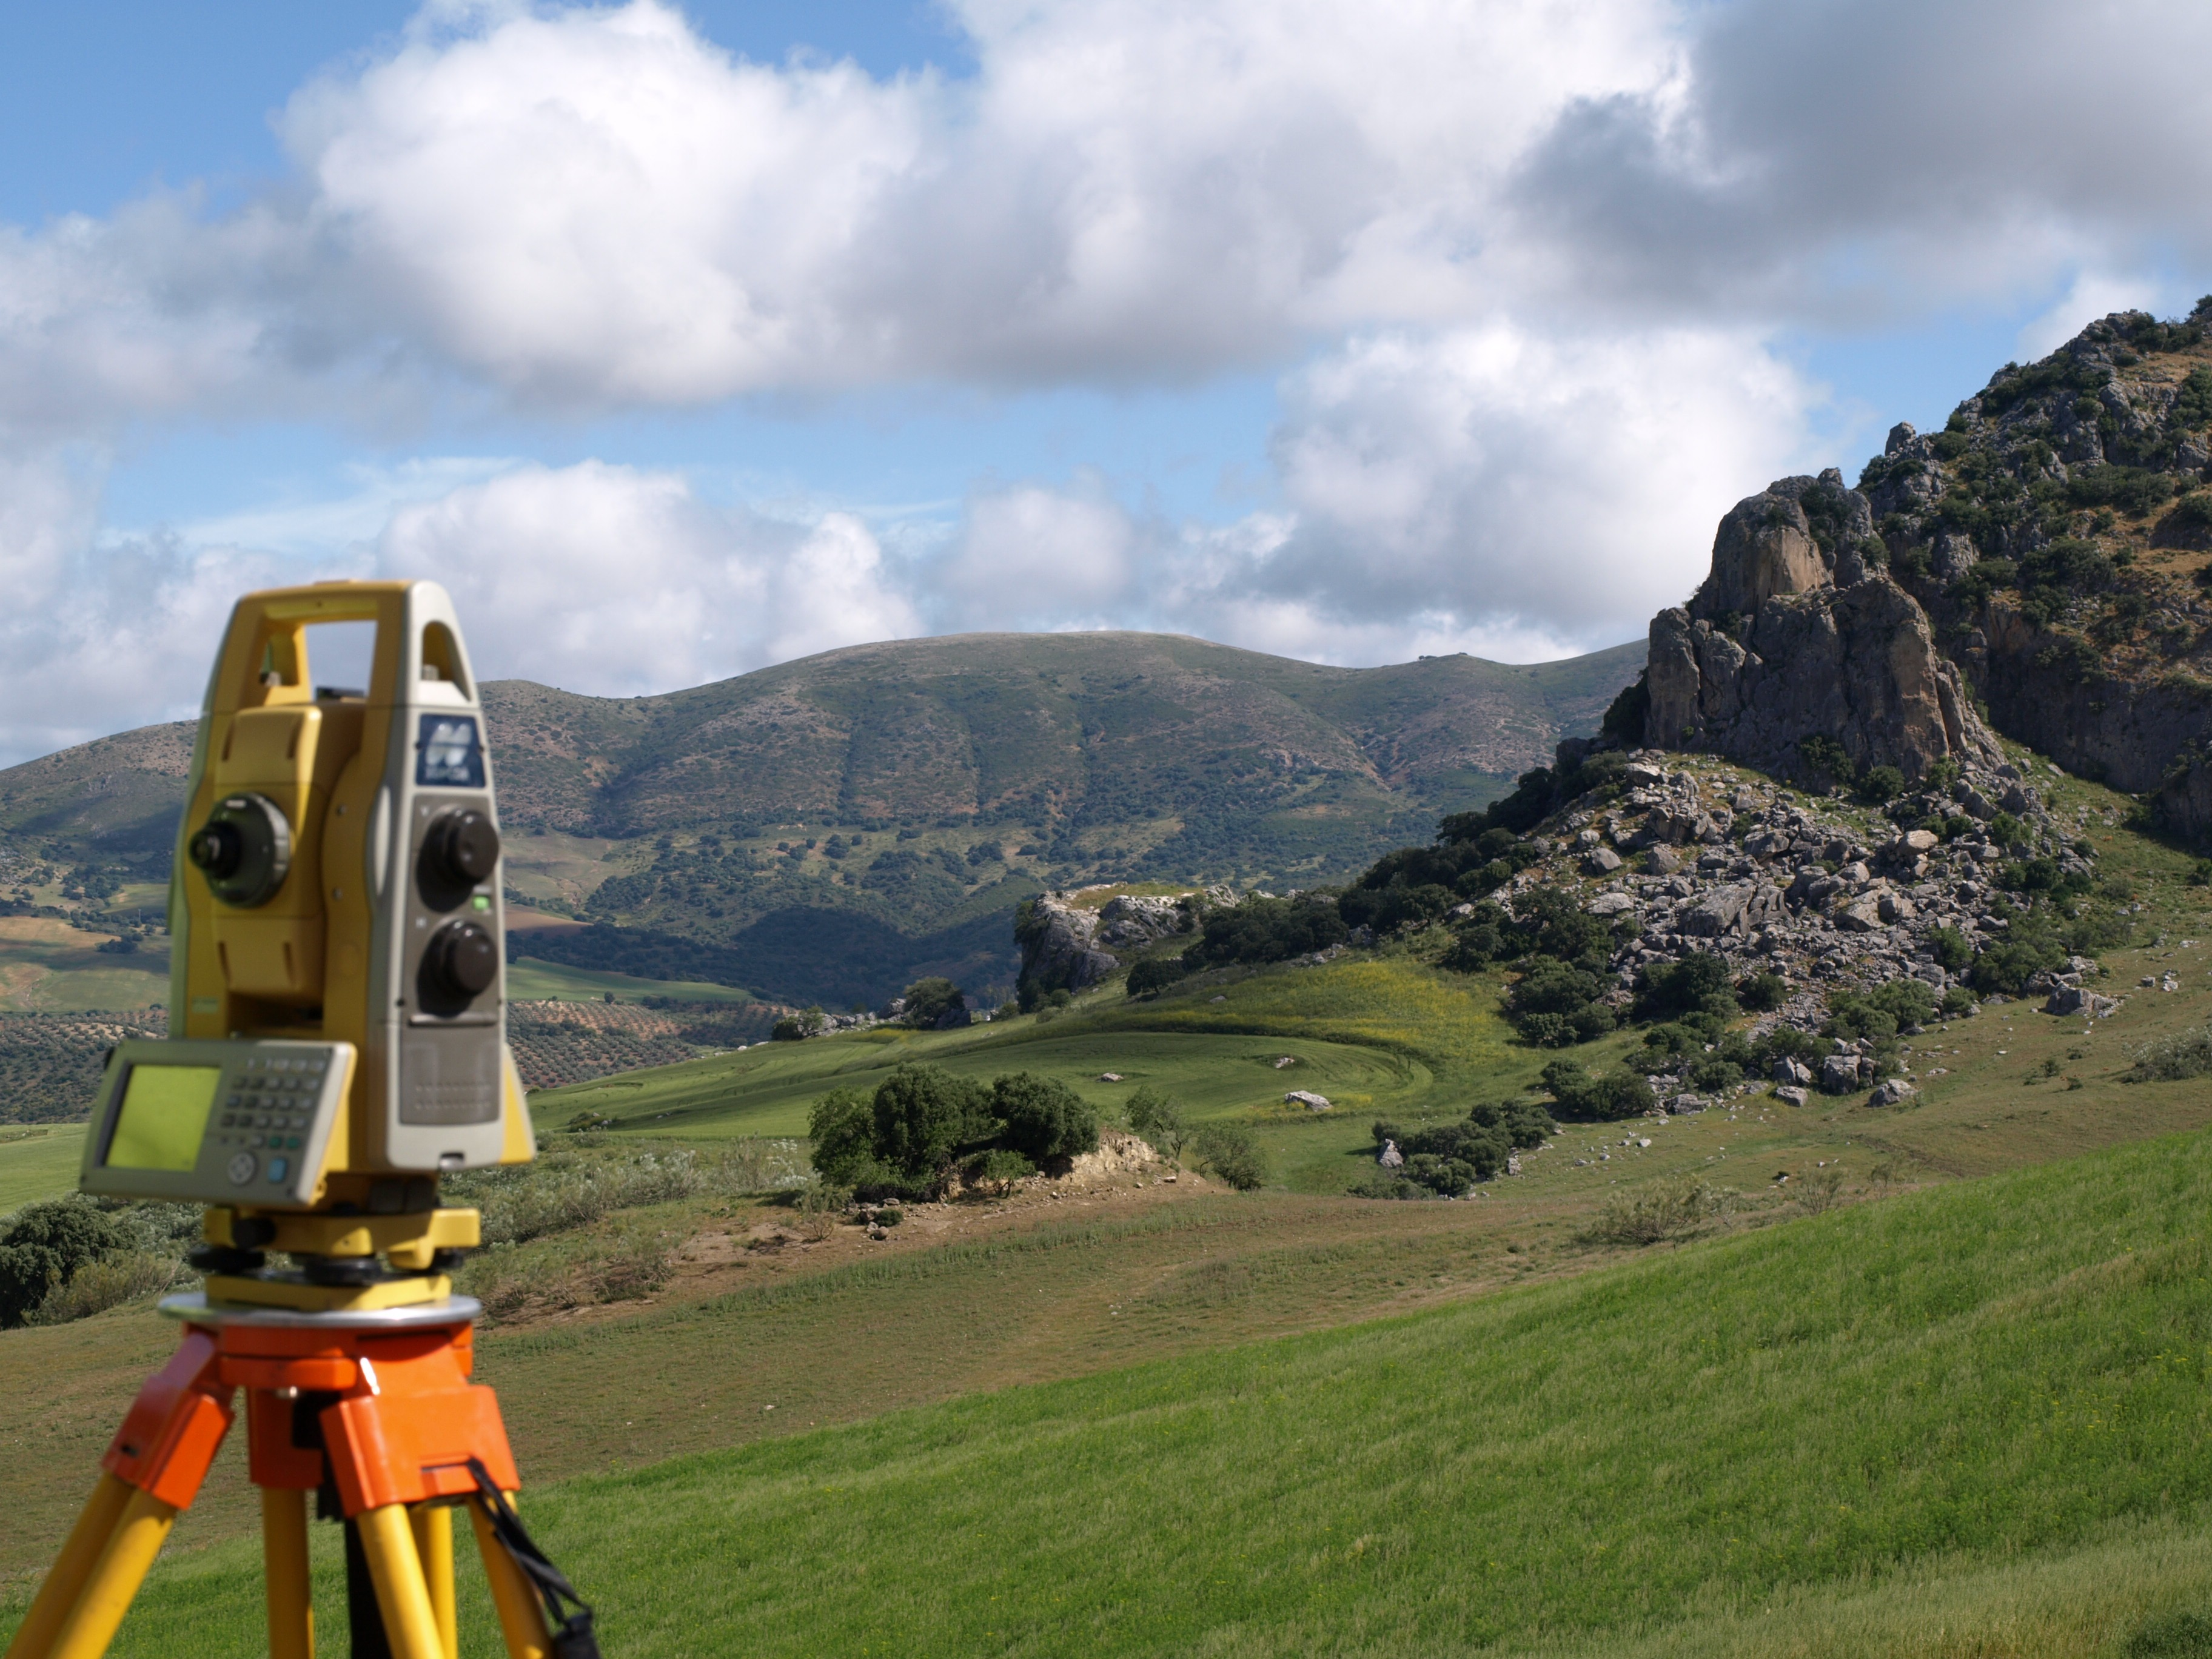
\includegraphics[width=\linewidth]{images/background}
		\end{column}%
	\end{columns}
	\note{say "hello" now}
\end{frame}